\begin{figure}[t]
    % Figures should be centered in the page/column
    \centering
    %
    \vspace*{-1em}
    %
    % Figure content goes here. This could be a graphic,
    % a TikZ diagram, etc.
    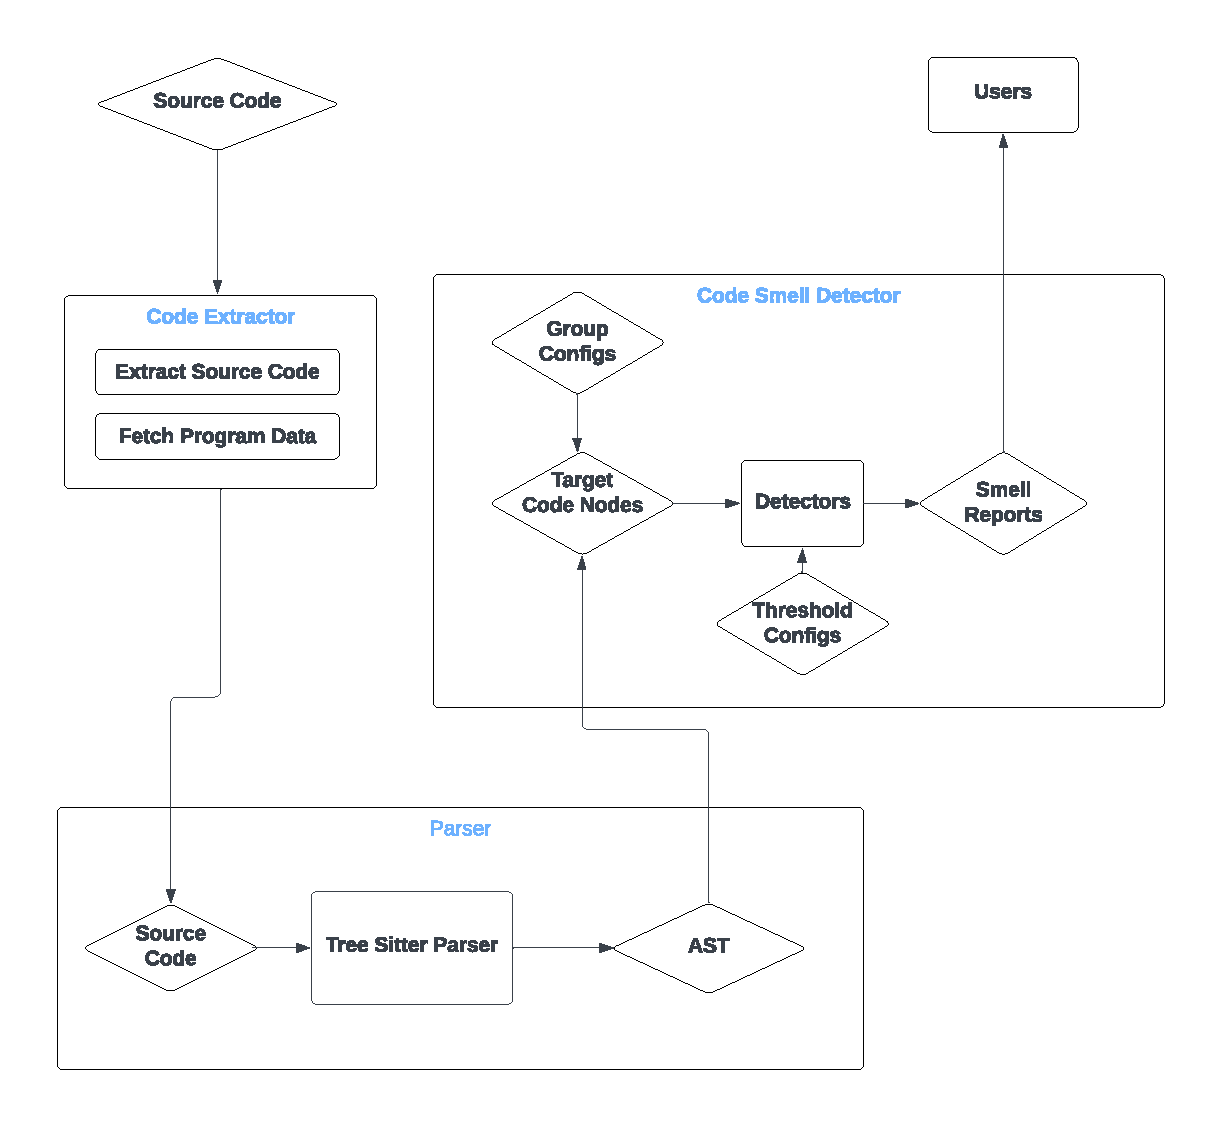
\includegraphics[width=\columnwidth]{graphics/Architecture.pdf}
    %
    \vspace*{-2em}
    %
    \caption{
        % The label should appear _inside_ the caption to ensure
        % Latex numbers it correctly. This is a common gotcha!
        %
        % All figure labels should start with "fig:"
        % So that the figure file can be found easily, the rest of the
        % figure label should be the same as the filename, as it is
        % in this example:
        %
        \label{fig:architecture}
        %
        The TreeNose tool for language-independent code smell detection.
    }
    \vspace*{-1.5em}
    %
    % To save space, you might want to remove space here
    % (use a negative \vspace, e.g. \vspace{-1em})
\end{figure}


% Use tight spacing around the title of the section

\vspace*{-0.5em}

\section{Language-Independent Smell Detection}~\label{sec:approach}

\vspace*{-1em}

% Give the basic definitions of the code smells
% Motivate why we picked these code smells
% Note: only four out of the five code smells that
% developers care about are implemented in TreeNose

{\bf Definitions}. Bearing in mind both the top 15 most common code smells
reported by developers~\cite{developersCare} and those smells commonly detected
by existing tools for Java, JavaScript, and Python, we designed
\texttt{TreeNose} to detect these code smells:

\begin{itemize}[leftmargin=*]
	%
    \item \textbf{Complex Conditional (CC)}~\cite{Fowler_Beck}: occurs when
        a conditional clause contains too many conditions, such as nested {\tt
        if-else} statements, and long {\tt switch-case} statements.
	      %
    \item \textbf{Long Class (LC)}~\cite{Fowler_Beck}: evident when a class
        defines too many (or too lengthy of) properties and/or behaviors.
	      %
    \item \textbf{Long Method (LM)}~\cite{Fowler_Beck}: a method has too
        many lines.
	      %
    \item \textbf{Long Message Chain (LMC)}~\cite{Fowler_Beck}: evident when
        there is a long chain of method calls and/or attribute references.
	      %
    \item \textbf{Long Parameter List (LPL)}~\cite{Fowler_Beck}: occurs when
        a method has too many input parameters.
	      %
\end{itemize}

% Describe each of the steps that TreeNose performs

{\bf Detection Technique}. Focused on the aforementioned code smells,
\texttt{TreeNose} uses Treesitter parsers and an AST-based approach to detect
code smells, as depicted in Figure~\ref{fig:architecture} and described in the
following list of smell detection steps:

\begin{itemize}[leftmargin=*]
    %
    % Step 1: Extract Source Code
    %
    \item \textbf{Step 1: Extract Source Code}: Extract source code written in
        the specified programming language, fetching every target file unless
        it or its containing path is in the ignore list.
        %
        % Step 2: Parse Source Code to AST; note the decoupling
        %
    \item \textbf{Step 2: Parse Source Code to AST}: Using Treesitter and its
        bindings for 18 languages, \texttt{TreeNose} parses the program's source
        code into an AST~\cite{treeSitter}. Adopting Treesitter decouples the
        parsing from the programming language's grammar, making it possible to
        parse multiple-language projects and various projects implemented in
        different languages.
        %
        % Step 3: Analyze AST to Detect Code Smells;
        % make sure to come clean about the manual mapping,
        % but make it clear that it is relatively simple
        %
    \item \textbf{Step 3: Analyze AST to Detect Code Smells}: To enable this
        automated step, we manually mapped the AST nodes reported by Treesitter
        to a simple, language-independent categorization, thereby enabling
        \texttt{TreeNose} to adopt the same detection process for nodes in the
        same group across multiple programming languages. During this step,
        \texttt{TreeNose} queries the AST and searches for the associated
        components. When it finds a component, like a method definition or a
        method call chain, \texttt{TreeNose} determines whether or not it is a
        code smell according to the thresholds given in
        Table~\ref{tab:metrics-and-thresholds}.
        %
\end{itemize}

% Tables should be placed at the top of pages/columns
% where they can.
%
% This can be ensured by using the [t] parameter to the
% "\begin{table}" declaration.
%
\begin{table}[t]
    % Figures should be centered in the page/column
    \centering
    %
    \caption{
        % The label should appear _inside_ the caption to ensure
        % Latex numbers it correctly. This is a common gotcha!
        %
        % All table labels should start with "tab:"
        % So that the figure file can be found easily, the rest of the
        % table's label should be the same as the filename, as it is
        % in this example:
        %
        \label{tab:metrics-and-thresholds}
        %
       Criteria thresholds for identifying smells with TreeNose.
    }
    %
    % Depending on the template, some breathing space might need to
    % be added (use \smallskip \medskip etc.) here
    %
    % Or, to save space, you might want to remove space
    % (use a negative \vspace, e.g. \vspace{-1em})
    %
    %
    % Table content goes here. Use this file to specify the
    % table's column headings. The data should be automatically
    % output from a program processing the raw experimental data
    % and should be inputted from another file. This enables
    % the data to change, if for example, the experiment data
    % needs to be updated.
    %
    % Do not use vertical rules. Ensure you use \toprule, \midrule
    % and \bottomrule from the "booktabs" package effectively.
    %
    % Numbers should be right justified (use "r"),
    % text left justified (use "l").
    %
    % For example:
    %
    \renewcommand{\arraystretch}{1.2}
    \begin{tabular}{@{}lll@{}}
        \toprule
            % use a new line for each column if needed
            {\bf Code Smell}
            &
            {\bf Criteria Threshold}
            &
            {\bf Metrics}
            \\
            %
        \bottomrule
        \input table-data/metrics
    \end{tabular}
    %
    % To save space, you might want to remove space here (use a negative
    % \vspace, e.g. \vspace{-1em})
    \vspace{-1em}
\end{table}

